\documentclass[UTF8]{ctexart}

\usepackage{hyperref}
\usepackage{syntonly}
\usepackage{graphicx}     
\usepackage{caption3}
\usepackage{subfigure}
\usepackage{float}        
\usepackage{listings}     
\usepackage{makeidx}
\usepackage[titles, subfigure]{tocloft}                 
\usepackage{enumitem}
\usepackage{tikz}
\usepackage{etoolbox}
\usepackage{geometry}
\usepackage{chngcntr}
\usepackage{amsmath}      
\usepackage{mathrsfs}   
\usepackage{bigstrut,multirow,rotating} 
\usepackage{longtable} 
\usepackage{graphicx}
\usepackage{titling}
\usepackage{url}
\graphicspath{
                {./figures/}
            }
\numberwithin{figure}{section}  
\numberwithin{table}{section}
\numberwithin{equation}{section}
\hypersetup{hidelinks,
	colorlinks=true,
	allcolors=black,
	pdfstartview=Fit,
    breaklinks=true}  
\renewcommand{\cftsecleader}{\cftdotfill{\cftdotsep}} 
\setlength{\parindent}{2em} 
\geometry{left=1.25in, right=1.25in,%
          top=1in, bottom=1in}
%%%%%%%%%%%%%%%%%%%%%%%%%%%%%%%%%%%%%%%%%%%%%%%%%%%%%%%%%%%%%

  
\begin{document}
    \title{
        \vskip 2cm \huge 金融中的优化与模拟方法22-23夏季 \\  
                    \huge 课程大报告 \\ 
                }

        \date{}
    \maketitle
    \clearpage

    \tableofcontents
    \clearpage

\section{摘要}
        本报告为\textbf{金融中的优化与模拟方法22-23夏季}课程的课程大报告,通过结合课程所学以及
    自身能力,本报告将主要针对下面两个问题给出一种朴素且简单的回答,力求在处理问题时增强自己对于
    课程所学知识的运用能力,并进一步增强对其的理解。本报告所关注的两个问题为:

        \begin{enumerate}
            \item 基于永续增长模型的自由现金流贴现方法计算长江电力(600900)的合理估值。
            \item 构建长江电力(600900)、贵州茅台(600519)、中国平安(601318)、中国国航(601111)
            的投资组合,并使用Markowitz均值-方差方法进行投资组合优化,使得在预期收益率年化20\%的
            情况下,其承担的风险最小。
        \end{enumerate}



\section{现金流贴现方法计算公司市值}
    \subsection{永续增长模型下的自由现金流贴现方法}
        永续增长模型指的是假设企业在此后经营状态稳定,有着固定的现金流增长率,且可以永续经营下去。基于此,
    如果已知企业某一年的现金流,并且能够通过某种方法估计出企业现金流的年增长率,那么就相当于知道了该企业
    今后每一年的现金流,通过乘以折现因子,就可以在该模型下计算出企业当前的内在价值。通过与当前企业市值的
    对比可以得到该企业目前市值是被高估、低估还是较好地反映了其内在价值。

        不妨设某公司当年的自由现金流为$CF$,现金流年增长率为$g$,贴现率为$r$,则下一年该公司的现金流折现为

        \begin{equation}
            CF_1 = \frac{CF \times (1+g)}{1+r}
        \end{equation}

        自然地,第二年的现金流折现为

        \begin{equation}
            CF_2 = \frac{CF \times (1+g)^2}{(1+r)^2}
        \end{equation}

        如此,当计及此后公司永续经营期间的所有现金流,并将其折现作为该公司的内在价值(不妨记为$P$),
    则有永续增长模型下的自由现金流贴现方法计算得到的公司内在价值:


        \begin{equation}
            \begin{aligned}
                P &= CF + \frac{CF \times (1+g)}{1+r} + \frac{CF \times (1+g)^2}{(1+r)^2} + \ldots \\
                    &= \lim_{n\rightarrow \infty} CF \frac{1 - \left(\frac{1+g}{1+r}\right)^n}{1-\left(\frac{1+g}{1+r}\right)} \\
                    &= CF \frac{1+r}{r-g}
            \end{aligned}
        \end{equation}

        一般地,对于该模型中的各个参数常采用以下估计方法:

        \begin{itemize}
            \item 年增长率$g$:对于一个处于长期稳定盈利的企业,可以认为其已经度过高速增长期
            而处于稳定盈利的状态,故年增长率不会太高,可取5\%到10\%的范围
            \item 贴现率$r$:一般采用加权平均资本成本(Weighted Average Cost of Capital, WACC)来计算,其中
            \begin{itemize}
                \item WACC = $\left(\frac{E}{V}\times Re\right) + \left(\frac{D}{V}\times Rd \times (1-T_c)\right)$
                \item $E$为公司市值
                \item $D$为公司债务市值
                \item $V = E+D$
                \item $Re$为公司的必要收益率(Required Rate of Return, RRR),$Re = Rf + b \cdot V$,其中
                \begin{itemize}
                    \item $Rf$为无风险收益率
                    \item $b$为投资者的风险价值系数,通常与投资者的风险偏好有关
                    \item $V$即标准离差率
                \end{itemize}
                \item $Rd$为债务成本
                \item $T_c$为企业税率
            \end{itemize}
        \end{itemize}

        通过以上的参数设定,结合企业当年的自由现金流,就可以求出在该模型下企业的内在估值了。

        下面以长江电力(600900)为研究对象,应用上述方法并结合其财务报表等信息,尝试计算其企业内在估值,并与
    其当前市值进行比较。

    \subsection{案例:长江电力(600900)}

        长江电力(600900)是沪深300指数成分股之一,在2023年6月21日更新的沪深300指数编排权重\footnote{\url{https://www.csindex.com.cn/\#/indices/family/detail?indexCode=000300}}中,其
    权重为1.14\%,为十大权重股之一。按中证行业分类为公用事业类公司。

        \begin{figure}[H]
            \centering
            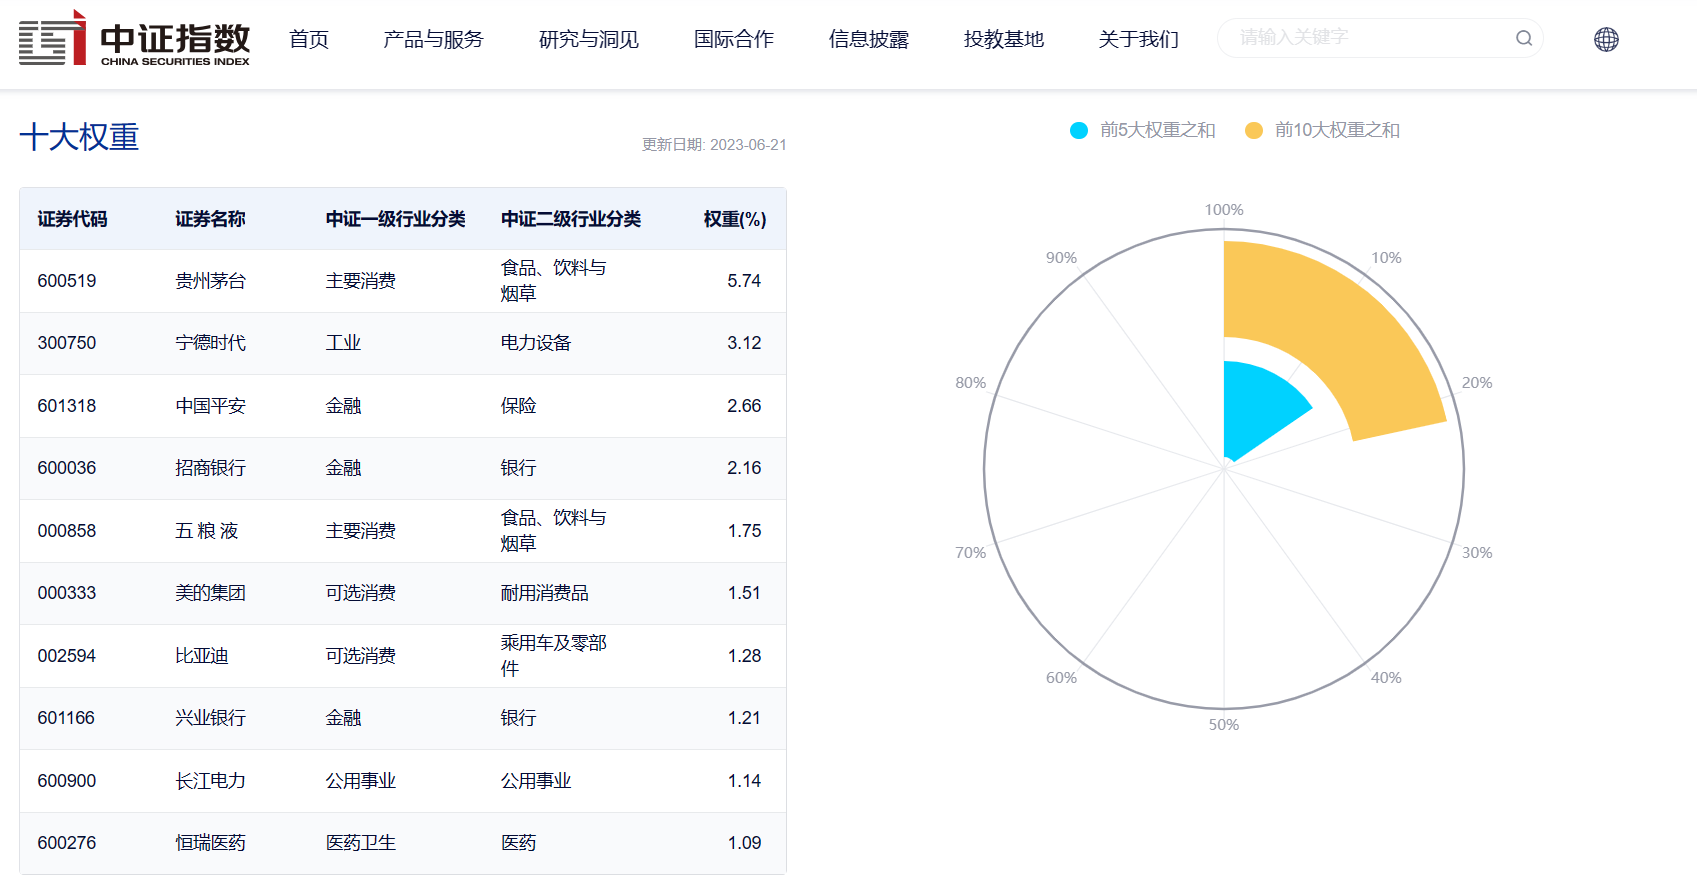
\includegraphics[width=0.8\textwidth]{Screenshot 2023-06-24 203818.png}
            \caption{2023年6月21日沪深300股指成分股十大权重}
        \end{figure}

        从公司官网,可见其经营业务主要为水电站的建设及其运营:

        \begin{figure}[H]
            \centering
            
\includegraphics[width=0.8\textwidth]{Screenshot 2023-06-24 204212.png}
            \caption{长江电力}
        \end{figure}

        作为公用事业公司,同时又是主营水电业务,可以预期其有着相当稳定的经营基础以及
    长期持续稳定盈利的能力,这也是选择其作为上一小节所述永续增长模型的自由现金流贴现方法
    的考察对象的重要原因。

        通过查看公司的财务报表,选择其中2022年扣除非经常性损益后的净利润作为初始现金流$CF=213.92$亿元,
    并估计其年增长率为$g=8\%$,而为了简化计算,取其净资产收益率(Rate of Return on Common Stockholders’ Equity, ROE)
    作为折现率(因折现率也可以理解为投资者的期望收益率,用ROE代替之作为估计),由已有数据可知,在2022年度报告
    后,其ROE为11.73\%,故取$r = 11.73\%$。

        则按照公式计算其内在价值为

        \begin{equation}
            \begin{aligned}
                P &= 213.92 \times \frac{1 + 11.73\%}{11.73\% - 8\%} \\
                    &\approx 6407 \text{亿元}
            \end{aligned}
        \end{equation}

        对比其当前市值(2023年6月24日)为5407亿,可知按照上述方法估计,该公司市值被低估了1000亿。


        
\newpage



\section{Markowitz均值方差方法优化投资组合}
    \subsection{Markowitz均值方差模型}
        按Markowitz均值方差方法,假定预设一个回报率$r_{\text{target}}$,对于不同的
    $n$个投资标的,可以按照如下问题求解来使得其风险最小:

    \begin{equation}
        \begin{aligned}
            \text{min} \quad & w^T \Sigma w \\
            s.t. \quad & w^T \mu \geq r_{\text{target}} \\
            & \sum_{i = 1}^{n}w_i = 1
        \end{aligned}
    \end{equation}

        其中,

        \begin{equation}
            \begin{aligned}
                w &= (w_1, w_2, \ldots, w_n)^T \\
                \mu &= (\mu_1, \mu_2, \ldots, \mu_n)^T
            \end{aligned}
        \end{equation}

        $w_i$为在第$i$个投资标的上分配资金的比例,$\mu_i$为第$i$个投资标的的
    年平均回报率,这里用其最近几年的平均年化来计算,而 

    \begin{equation}
        \Sigma=\left[\begin{array}{ccc}
        \sigma_{11} & \cdots & \sigma_{1 n} \\
        \vdots & \ddots & \vdots \\
        \sigma_{n 1} & \cdots & \sigma_{n n}
        \end{array}\right]
    \end{equation}

        其中,$\sigma_{ij}$为第$i$个投资标的与第$j$个投资标的之间的协方差,
    $\Sigma$即协方差矩阵。

    \subsection{案例:四只股票投资组合中Markowitz均值方差模型的应用}

        由于投资组合的选取是用来对冲股票的非系统性风险的,故尽可能选取不同行业的
    股票作为投资组合中的投资标的,这里我们选取长江电力(600900)、贵州茅台(600519)、中国平安(601318)、中国国航(601111)
    这四只股票进行投资组合构建,其分别属于公用事业、主要消费、非银金融与航空运输,且上市时间均早于2008年,分析中
    选取其自2009年至今的股价表现进行上述计算(因长江电力曾于2008年5月经理长达一年的停牌,故从2009年开始算起)。

        首先,从东方财富网获取四只股票按年计的价格表现,并计算出其每年的年化收益。其中,股票行情的
    抓取是通过开源项目\href{https://akshare.akfamily.xyz/index.html}{AKShare}提供的接口实现的。
    相应源代码可见\textbf{../src/save\_data.py}。由于行情接口的限制,最多只能抓取月线数据,
    故实际处理中从月线数据算出每年的收益率再进行下一步处理。下载到的月线数据保存在\textbf{../data}
    目录中。通过处理,得到各支股票从2009年到2022年各年度的收益率为:

    \begin{table}[H]
        \centering
        \begin{tabular}{|c|c|c|c|c|}
        \hline
            & 600900       & 600519       & 601318        & 601111       \\ \hline
        2010 & -10.97701149 & 8.7968538    & 2.69694819    & 40.38657172  \\ \hline
        2011 & -10.78114913 & 16.40233138  & -36.5756738   & -52.10144928 \\ \hline
        2012 & 9.69609262   & 9.85544228   & 30.6456007   & -3.93343419  \\ \hline
        2013 & -2.50659631  & -33.77050258 & -6.38031693   & -31.33858268 \\ \hline
        2014 & 54.8037889   & 58.10379341  & 75.0111359    & 90.36697248  \\ \hline
        2015 & 25.04370629  & 26.17480564  & -2.35428862  & 9.51807229   \\ \hline
        2016 & -2.27193289  & 50.89315332  & -0.0521308484 & -13.97139714 \\ \hline
        2017 & 26.96709585  & 102.2137585  & 92.8413092    & 66.8797954   \\ \hline
        2018 & 4.76056338   & -13.17627618 & -16.3094192  & -35.01915709 \\ \hline
        2019 & 14.97714439  & 95.56023715  & 50.4322534   & 25.35377358  \\ \hline
        2020 & 5.98690365   & 66.92144544  & 3.88850099    & -20.22577611 \\ \hline
        2021 & 16.37246249  & 3.43527043   & -35.4546864   & 19.33962264  \\ \hline
        2022 & -2.93894577  & -13.01659616 & -1.58590308   & 14.5256917   \\ \hline
        \end{tabular}
        \caption{各支股票的年度收益率,单位取\%}
    \end{table}

    由此,可计算出各支股票的平均年度收益率$\mu$为:
    \begin{table}[H]
        \centering
        \begin{tabular}{|c|c|c|c|}
        \hline
        600900     & 600519      & 601318      & 601111     \\ \hline
        9.93324015 & 29.10720896 & 12.06179456 & 8.44466949 \\ \hline
        \end{tabular}
        \caption{各支股票的平均年度收益率,单位取\%}
    \end{table}

    以及其协方差矩阵$\Sigma$为:
   
    \begin{table}[H]
        \centering
        \begin{tabular}{|c|c|c|c|}
        \hline
        331.40575167 & 374.36518216  & 483.42970976  & 538.35962166  \\ \hline
        374.36518216 & 1802.8362803  & 1196.19035852 & 863.13969198  \\ \hline
        483.42970976 & 1196.19035852 & 1564.11578491 & 1233.19200097 \\ \hline
        538.35962166 & 863.13969198  & 1233.19200097 & 1683.69145254 \\ \hline
        \end{tabular}
        \caption{协方差矩阵}
    \end{table}

        有了以上信息,就可以求解在上一小节中所描述的问题了。其中优化求解使用的
    是python的开源项目\href{https://www.cvxpy.org/index.html}{CVXPY},实现
    代码可见\textbf{../src/portfolio.py}。通过构建问题并求解,最终解得如下
    投资组合选择:

    \begin{table}[H]
        \centering
        \begin{tabular}{|c|c|c|c|}
        \hline
        600900 & 600519 & 601318 & 601111 \\ \hline
        47.5\% & 52.5\% & 0      & 0      \\ \hline
        \end{tabular}
        \caption{在Markowitz均值方差模型下求解的投资组合}
    \end{table}

        可见,在保证平均年化收益不低于20\%的条件下,模型倾向于选择长江电力(600900)
    与贵州茅台(600519)来进行投资组合,其中前者是增长较稳定的公用事业水电公司,
    而后者的回报率虽然存在一定的周期因素,但往往能够在行情较好时给予投资者超额回报。
    同时应当注意的是,从协方差矩阵中可以看出,选择的四至股票之间的协方差均为非负数,
    这说明只选择股票作为投资组合的投资标的仍存在其局限性。此后如果将固收类资产
    也考虑到投资组合的选取中,则有望进一步降低风险。

    \section{结语}
        本报告主要结合课程讲授内容中的两处知识点进行讨论,并结合假想的简单案例
    尝试动手应用课程所学知识。在处理问题的过程中,重温了课程所学,并结合自主的
    探索,学习到了很多此前所不知道的知识和技巧。不过限于报告作者对于金融领域中
    专业知识的匮乏,文中可能出现纰漏或错误,恳请不吝指正!






\end{document}